\documentclass[sigconf,10pt]{acmart}

\usepackage[boxed]{algorithm2e}
\usepackage{tikz}
\usetikzlibrary{cd, positioning}

\graphicspath{{img/}}

\newtheorem{definition}{Definition}[section]

\usepackage{amsmath}
\usepackage{amsfonts}
\usepackage{amssymb}
\usepackage{multirow}
\usepackage{array}
\usepackage{subcaption}
\usepackage{mathtools}
\usepackage{listings}
\usepackage{subcaption} %https://tex.stackexchange.com/questions/365198/idiomatic-approach-to-captioned-subfigures-and-tables-with-the-2017-acmart-class
\usepackage{tikz} 
\newcolumntype{L}{>{$}l<{$}}
\DeclareMathOperator{\map}{map}
\DeclareMathOperator{\im}{im}
\DeclareMathOperator{\toList}{toList}
\DeclareMathOperator{\toSet}{toSet}
\DeclareMathOperator{\toBag}{toBag}
\DeclareMathOperator{\isGraphBag}{isGraphBag}
\DeclareMathOperator{\sort}{sort}
\DeclareMathOperator{\concat}{concat}
\DeclareMathOperator{\canonizeGraphBag}{canonizeGraphBag}
\newcommand{\unbind}[1]{{\ensuremath{\scriptstyle\left[-#1\right]\,}}}
\newcommand{\bind}[1]{{\ensuremath{\scriptstyle\left[#1\right]\,}}}

\newcommand{\lrparen}[1]{% \lrparen{..}
  \left(#1\right)}
\newcommand{\lrcurly}[1]{
  \left\{#1\right\}}
\newcommand{\lrbracket}[1]{
  \left[#1\right]}
\newcommand{\lrceil}[1]{
  \left\lceil#1\right\rceil}
\newcommand{\llrrbracket}[1]{
  \left[\mkern-3mu\left[#1\right]\mkern-3mu\right]}
\newcommand{\llrrparen}[1]{
  \left(\mkern-6mu\left(#1\right)\mkern-6mu\right)}
\newcommand{\lrangle}[1]{
  \left\langle#1\right\rangle}

\newcommand{\Bold}[0]{B_{old}}
\newcommand{\Bcur}[0]{B_{cur}}
\newcommand{\Bnew}[0]{B_{new}}
\newcommand{\MPLAN}[0]{\textsc{MPlan}}
\newcommand{\RPLAN}[0]{\textsc{RPlan}}


% \usepackage[utf8]{inputenc}
% \usepackage{booktabs} % For formal tables
% Copyright
%\setcopyright{none}
%\setcopyright{acmcopyright}
%\setcopyright{acmlicensed}
\setcopyright{rightsretained}
%\setcopyright{usgov}
%\setcopyright{usgovmixed}
%\setcopyright{cagov}
%\setcopyright{cagovmixed}

% DOI
% \acmDOI{10.475/123_4}

% ISBN
% \acmISBN{123-4567-24-567/08/06}

%Conference
\acmConference[SIGMOD]{ACM SIGMOD}{June 2019}{Amsterdam, NL} 
\acmYear{2019}
\copyrightyear{2019}


% \acmArticle{4}
\acmPrice{15.00}


\newcommand{\tr}[0]{{\mathsf{T}}}

\begin{document}
\title{Wormhole: Sum-Product Optimization for Large-Scale Linear Algebra}
\author{Shana Hutchison}%
\orcid{0000-0002-3206-3415}
\email{shutchis@cs.washington.edu}
\author{Jonathan Leang}
\email{jleang@cs.washington.edu}
\author{Remy Wang}
\email{remywang@cs.washington.edu}
\author{Bill Howe}
\email{billhowe@uw.edu}
\author{Dan Suciu}
\email{suciu@cs.washington.edu}
\affiliation{%
  \institution{University of Washington}
    \city{Seattle} 
    \state{Washington} 
    \postcode{98195}
    \country{USA}
}
\author{Alexandre Evfimievski}
\email{evfimi@us.ibm.com}
\author{Berthold Reinwald}
\email{reinwald@us.ibm.com}
\author{Prithviraj Sen}
\email{senp@us.ibm.com}
\affiliation{%
  \institution{IBM Research -- Almaden}
    \city{San Jose} 
    \state{California} 
    \postcode{95120}
    \country{USA}
}
\author{Matthias Boehm}
\email{m.boehm@tugraz.at}
\affiliation{%
  \institution{Technische Universit\"{a}t Graz}
    \city{Graz}
    \country{Austria}
}

\renewcommand{\shortauthors}{Hutchison, Leang, Howe, Suciu, Evfimievskit, Reinwald, Sen, Boehm}

\begin{abstract}
Machine learning algorithms are commonly specified in linear algebra.
These algorithms can be rewritten into more efficient forms, 
by taking advantage of the properties of their underlying sum 
and product operations.
However, existing optimization algorithms fail to fully search through the large space of equivalent sum-product expressions and find the best version to run, due to challenges lying in the addition operation and common sub-expressions (CSEs).
In this paper, we introduce a cost-based optimization technique for selecting the best alternative in linear algebra scripts that include the plus, multiply, and aggregation operators as well as CSEs.
Our experiments in SystemML show competitive performance alongside existing optimization heuristics across a spectrum of machine learning tasks, as well as large speedups in cases where newfound rewrites apply.
\end{abstract}

% %
% % The code below should be generated by the tool at
% % http://dl.acm.org/ccs.cfm
% % Please copy and paste the code instead of the example below. 
% %
% \begin{CCSXML}
% <ccs2012>
%  <concept>
%   <concept_id>10010520.10010553.10010562</concept_id>
%   <concept_desc>Computer systems organization~Embedded systems</concept_desc>
%   <concept_significance>500</concept_significance>
%  </concept>
%  <concept>
%   <concept_id>10010520.10010575.10010755</concept_id>
%   <concept_desc>Computer systems organization~Redundancy</concept_desc>
%   <concept_significance>300</concept_significance>
%  </concept>
%  <concept>
%   <concept_id>10010520.10010553.10010554</concept_id>
%   <concept_desc>Computer systems organization~Robotics</concept_desc>
%   <concept_significance>100</concept_significance>
%  </concept>
%  <concept>
%   <concept_id>10003033.10003083.10003095</concept_id>
%   <concept_desc>Networks~Network reliability</concept_desc>
%   <concept_significance>100</concept_significance>
%  </concept>
% </ccs2012>  
% \end{CCSXML}

% \ccsdesc[500]{Computer systems organization~Embedded systems}
% \ccsdesc[300]{Computer systems organization~Redundancy}
% \ccsdesc{Computer systems organization~Robotics}
% \ccsdesc[100]{Networks~Network reliability}

% \keywords{ACM proceedings, \LaTeX, text tagging}

\maketitle

% \section{Introduction}
Large-scale machine learning (ML) aims at statistical analysis and predictive modeling over large data collections~\cite{CohenDDHW09}, commonly using data-parallel frameworks like Spark~\cite{ZahariaCDDMMFSS12}. State-of-the-art ML systems allow data scientists to express their ML algorithms---ranging from classification, regression, and clustering to matrix factorization and deep learning---in linear algebra and statistical functions \cite{AbadiBCCDDDGIIK16,BoehmDEEMPRRSST16,HuangB013,LuoGGPJ17,RohrmannSRG17,MahoutSamsara,StonebrakerBPR11,YuSC15,YuTAMAO17}, and automatically compile efficient execution plans. This high-level specification simplifies the development of custom ML algorithms, and allows the adaptation of execution plans to different data, hardware, and deployment characteristics.


\paragraph{Rewriting Opportunities in Linear Algebra} 
As the lingua franca of ML algorithms, linear algebra admits numerous rewriting opportunities that improve their performance.  For example, the rewrites XXXX 

The rewrites listed above are just a small selection of useful rewrites to include inside a query optimizer for ML algorithms.  An immediate question to address is whether we can write down \emph{every} linear algebra rewrite that improves ML algorithm performance. Many ML optimizers (e.g., X, Y, Z) aim to achieve exactly this, encoding long lists of rewrite rules that encode identities as well as the conditions and order in which to apply them.

Unfortunately, exhaustively enumerating linear algebra identities that improve performance in rule-based optimizers is a significant challenge.  Newly written ML scripts admit new patterns of linear algebra operators, which often require adding rewrite rules and re-thinking the order in which they apply (often called the phase ordering problem \cite{X}).


\paragraph{A ``Primitive'' Approach to LA Rewrites}
The core of these rewrites lies not in matrix identities but instead in properties of the primitive scalar operators + and *.  These scalar operators are the basis of the most common linear algebra operators including matrix addition ($A + B$), matrix multiplication ($AB$), element-wise multiplication ($A * B$), and aggregation (sum($A$), rowSums($A$), colSums($A$)).

In this work, we build on the hypothesis that reasoning at the scalar level inside an optimizer will match the performance of existing rule-based optimizers, by deriving their identities from first principles, as well as exceed their performance in some cases via the automatic derivation of new identities.


\paragraph{An Example from Matrix Factorization}
Consider the task of Gaussian matrix factorization.  
This task factorizes a matrix $X$, often sparse, into the product of low-rank dense matrices $UV^\tr$. 
Matrices $U$ and $V$ are iteratively updated until the difference between $X$ and its approximation is small enough in L2, $sum((X - UV^\tr)^2) < \epsilon$.  The ``power of 2'' operator here indicates element-wise power, i.e., raising each entry of the matrix to the power 2.

The query $sum((X - UV^\tr)^2)$ is expensive even for moderately sized matrices. 
The problem is that $UV^\tr$ creates a dense intermediary in the shape of $X$, even though $X$ is sparse, resulting in high memory and CPU pressure.
The LA engines SystemML (0.14), XXX, and YYY all struggle to execute this query, not because the query is impossible to optimize but rather that their optimizers are missing a rule that targets this pattern.

A rewrite of this query into a more efficient form can be recovered from first principles as follows:
\begin{enumerate}
  \item Decompose subtraction into addition:\\ $sum((X + (-1)*UV^\tr)^2)$.
  \item Decompose element-wise power into element-wise multiplication: 
  $sum((X + (-1)*UV^\tr) * (X + (-1)*UV^\tr))$.
  \item Rewrite matrix operators as scalar operators over indexed matrices: 
  $\sum_{ik} ((X_{ik} + \sum_j (-1)*U_{ij}V_{kj}) * (X_{ik} + \sum_l (-1)*U_{il}V_{kl}))$.
  \item Distribute $*$ over $+$ and $\sum$ over $+$; factor $\sum$ from $*$: 
  $\sum_{ik} X_{ik}*X_{ik} + \sum_{ikj} (-2)*X_{ik}*U_{ij}V_{kj} + \sum_{ikjl} U_{ij}V_{kj}*U_{il}V_{kl}$.
  \item Reorder aggregated indices in the third term and factor:
  $\sum_{ik} X_{ik}*X_{ik} + \sum_{ikj} (-2)*X_{ik}*U_{ij}V_{kj} + \sum_{jl} (\sum_i (U_{ij}U_{il}) * \sum_k (V_{kj}*V_{kl}))$.
  \item Recover matrix operators, subtraction, power:\\
  $sum(X^2) - 2*sum(X*UV^\tr) + sum(U^\tr U * V^\tr V)$.
\end{enumerate}
The final expression exploits the sparsity of $X$ in the first two terms\footnote{$X$ multiplies with $UV^\tr$ in the rewritten plan, allowing the computation to proceed only in the non-zero entries of $X$, whereas $X$ subtracts $UV^\tr$ in the original expression to form a dense matrix.}, and it converts the third term into the element-wise multiplication of inner products, which are far smaller than the outer product $UV^\tr$.\footnote{To relate these steps to our optimizer, steps 1--4 rewrite the query into a canonical form (see Section 2), from which the factorization in step 5 is found during search.}

While any rule-based optimizer could encode a rule for this rewrite directly (in fact, SystemML added such a rule in version 0.15), we highlight how it automatically arises as a result of primitive rewrites at the scalar level. In general, however, generating rewrites from first principles is more risky than taking a rule-based optimization approach.  The challenge lies in the large search space generated by rewrites at the primitive level; there is no guarantee that a good rewrite can be found in a reasonable time frame.  

% missing DAG challenges CSE

\paragraph{Contributions}
We introduce a cost-based framework for optimizing the sum-product portions of linear algebra scripts.  In particular, the framework optimizes expressions containing addition and common sub-expressions (CSEs), on top of multiplication and aggregation as covered by previous work.  The framework revolves around a canonical form defined on an indexed-matrix representation, from which it explores alternative rewrites within a carefully carved search space.  

Section 2 -- related work

Section 3 -- representation and canonical form

Section 4 -- search strategy and pruning

Section 5 -- experiments

We prototype our framework in Apache SystemML, a large-scale LA execution engine.  However, we believe that our techniques apply more generally to other LA engines, such as Tensorflow and Julia, when given reasonable cost models over their operators.




\section{Related Work}
The closest sum-product optimization frameworks in the literature (FAQ \cite{KhamisNR16}, AJAR \cite{Joglekar2016AJARAA}, PANDA) cover LA expressions involving $*$ and $\sum$.
These frameworks have an excellent coverage of theory and implementation,
but they fall short of LA workloads that occur in practice.
We step past these frameworks by (1) incorporating common sub-expressions and (2) incorporating addition ($+$).

...


\section{Modeling the Optimization Problem}

Linear algebra means one data type (matrix) and a set of matrix operations:
%\begin{align*}
%M * M \rightarrow M & \text{elemmult} \\
%M + M \rightarrow M & \text{elemplus} \\
%MM \rightarrow M & \text{mmult} \\
%\sum_{row} M \rightarrow M & \text{rowagg} \\
%\sum_{col} M \rightarrow M & \text{colagg} \\
%\sum M \rightarrow M & \text{agg} \\
%% M^k \rightarrow & \text{power} \\
% M^\tr & \text{transpose} \\
% \end{align*}


% \begin{table}[]
% \begin{tabular}{lll}
% name & type & syntax \\
% \hline
% mmult & $M_{N,L} \times M_{L,M} \rightarrow M_{N,M}$ & $AB$  \\
% elemmult & $M_{N,M} \times M_{N,M} \rightarrow M$ & $A*B$ \\
% elemplus & $M_{N,M} \times M_{N,M} \rightarrow M_{N,M}$ & $A+B$ \\
% rowagg & $M_{N,M} \rightarrow M_{N,1}$ & $\sum_{row} A$ \\
% colagg & $M_{N,M} \rightarrow M_{1,M}$  & $\sum_{col} A$ \\
% agg & $M_{N,M} \rightarrow M_{1,1}$ & $\sum A$ \\
% %power & $M  \times Int \rightarrow M$ & $A^k$ \\
% transpose & $M_{N,M} \rightarrow M_{M,N}$ & $M^\tr$ \\
% \end{tabular}
% \end{table}

This language subsumes most definitions of linear algebra.   Matrix multiply is modeled as elemmult followed by aggregation.   FAQ was just elemult and aggregation, not elemplus. 

Example: AB + AC + AD + AE = A(B+C+D+E)   RHS is clearly faster (only one multiply) if A is dense.

1) Nobody else does this kind of reasoning.  (caveats?)
2) This kind of reasoning is hard, because the space blows up.  (evidence?  Can we analytically derive the blowup?)
3) This kind of reasoning matters.  Besides Example 1, we find that this kind of reasoning can lead to plans that are X times faster than plans optimized without considering elemplus.  This matters, part 2: Does it show up in practice?  Yes: Consider any ML algorithm -- regularizers, errors, update rules all have combinations of sums and products.

with existing heuristics

Optimization problem is to find an equivalent expression with a lower estimated cost.

[Some things to show somewhere that cost model reflects true costs]

Figure: "Symbols used"

%SumProduct Expression:
%mmult, elemmult, elemplus, elemminus, elempower, $\Sigma$, transpose


%A DimLabel with respect to a tensor or indexed tensor A is an injective function mapping the dimensions of A to a universe of labels. 
%$Bind_{i,j}(A)$ assigns the label $i$ to the first dimension of A (its rows), and $j$ to the second dimension (its columns).


\section{Plan Representation}
In this section we define sum-product matrix expressions (the input and output of our optimizer), SPlans (the primitive decomposition our optimizer reasons with), a canonical form for SPlans (used to stage cost-based search), and the graph representation of SPlans (used to define the search procedure).


\subsection{Sum-Product Matrix Expressions}
The programs that SystemML compiles are specified in the DML, a syntax similar to R.  The scope of DML is much larger than the scope of this paper, due to the presence of advanced operators such as cbind (concatenate the columns of two matrices), table (construct a matrix from vectors of column indices, row indices, and values), element-wise Boolean functions, and control-flow operators (e.g. if statements, while loops).
For the purpose of this paper, we narrow our optimizer to a single control-flow unit and to ignore advanced operators, treating them instead as black-box external functions.

The fragment of DML paired-down to the operators we wish to optimize can be defined as sum-product matrix expressions:
\begin{definition}[Sum-product matrix expression]
In the following, let the term ``matrix'' refer also to vectors and scalars, but not higher-order tensors.
A sum-product matrix expression is a collection of expressions (one for each output) in an algebra over matrices with the following operators:
\begin{itemize}
  \item Unary operators: element-wise power (parameterized with a constant, non-negative integer power), aggregation (parameterized with an aggregation type: row, column, or both), and transpose.
  \item Binary operators: matrix multiply, element-wise multiply, addition, and subtraction.
  \item N-ary operators: external functions treated as black boxes.
\end{itemize}
\end{definition}


Take the example of computing the means and variances of the columns from the matrix multiplication $AB$ as an example.
This can be written as the sum-product matrix expression $colSums(AB) / nrow(A),\; (colSums((AB)^2) - colSums(AB)^2) / nrow(A)$, where $nrow$ is an external function that returns the number of rows in a matrix (usually inlined) and $/$ is an external function that computes element-wise division.

Figure XX presents this sum-product matrix expression in DAG form.
It is conventient to write sum-product as DAGs because they emphasize the presence of common sub-sxpressions (CSEs), which are critical to recognize during optimization.  
This particular DAG has two roots for the output row vectors.

%The next section continues with this example, translating the sum-product matrix expression into an SPlan.
% also present: dimension, shape, sparsity estimate



\subsection{SPlans}
While sum-product matrix expressions correctly capture the semantics of a ML algorithm, it is difficult to reason over them directly because they contain compound operators like matrix multiplication and element-wise power.  In this section we introduce SPlans as the decomposition of sum-product matrix expressions.  First we define the objects of SPlans, indexed tensors, and then define SPlans and include an example.

\begin{definition}[Indexed Tensor]
An indexed tensor is a tensor with a different index for each of its dimensions.
The set of indices of an indexed tensor is called its \emph{schema}.
The set inclusion $i \in A$ denotes that the index $i$ is present in the schema of a tensor $A$.
Each index has an associated natural number shape, denoted $|i|$ for an index $i$. 
An indexed tensor's shape is defined by the shape of the indices in its schema.
\end{definition}
For example the matrix $A$ may be assigned the index $i$ over its rows and $j$ over its columns, to be written as $A_{ij}$.
While the order in which indices are assigned to dimensions is significant, the schema itself is unordered.

\begin{definition}[SPlan]
An SPlan is a collection of expressions (one for each output) in an algebra over tensors and indexed tensors with the following operators:
\begin{itemize}
  \item Unary operators: bind (assign indices to an tensor), unbind (unassign indices from an indexed tensor), aggregation (over an indexed tensor; parameterized with the indices to aggregate).
  \item N-ary operators: multiply, addition (both over indexed tensors), external functions treated as black boxes (over tensors).
  \begin{itemize}
    \item The arguments of multiply and addition are unordered.
  \end{itemize}
\end{itemize}
\end{definition}


\begin{table}[]
\begin{tabular}{llll}
&name & type & syntax \\
\hline
\multirow{7}{*}{\rotatebox[origin=c]{90}{MPlan}} 
&mmult & $T_{M,L} \times T_{L,N} \rightarrow T_{M,N}$ & $AB$  \\
&elemmult & $T_{M,N} \times T_{M,N} \rightarrow T_{M,N}$ & $A*B$ \\
&elemplus & $T_{M,N} \times T_{M,N} \rightarrow T_{M,N}$ & $A+B$ \\
&rowagg & $T_{M,N} \rightarrow T_{M,1}$ & $\sum_{row} A$ \\
&colagg & $T_{M,N} \rightarrow T_{1,N}$  & $\sum_{col} A$ \\
&agg & $T_{M,N} \rightarrow T_{1,1}$ & $\sum A$ \\
%&power & $M  \times Int \rightarrow M$ & $A^k$ \\
&transpose & $T_{M,N} \rightarrow T_{N,M}$ & $A^\tr$ \\
\hline
\multirow{2}{*}{\rotatebox[origin=c]{90}{conv.}}
&bind & $T_{M,N} \times [i,j] \rightarrow R_{i:M,j:N}$ & $\bind{i,j} A$ \\
&unbind & $R_{i:M,j:N} \times [i,j] \rightarrow T_{M,N}$ & $\unbind{i,j} A$ \\
\hline
\multirow{2}{*}{\rotatebox[origin=c]{90}{SPlan}}
&join & $R_{S_1} \times R_{S_2} \rightarrow R_{S_1 \cup S_2}$ & $A*B$ or $A+B$ \\
&agg & $R_S \times U \rightarrow R_{S \setminus U}$ & $\sum_{U} A$ \\
\end{tabular}
\caption{Operators used in MPlans and SPlans. Uninterpreted black-box functions are also allowed.}
\end{table}


SPlans decompose and assign indices to the parts of a sum-product matrix expression that can be optimized by rewrites over addition, multiplication, and aggregation.  The parts that cannot be optimized does not use indices and remains outside the purview of the optimizer.

Translating a sum-product matrix expression to an SPlan is a straightforward application of a few rules:
\begin{enumerate}
  \item $A - B \rightarrow A + (-1) * B$
  \item For small non-negative integers $k$, $A^k \rightarrow A * A^{k-1}$.
  \item $A*B \rightarrow Unbind_{i,j}(Bind_{i,j}(A)*Bind_{i,j}(B))$.  \\Same pattern for $+$.
  \item $AB \rightarrow Unbind_{i,k} \sum_j (Bind_{i,j}(A)*Bind_{j,k}(B))$. 
  \item $A^\tr \rightarrow Unbind_{j,i}(Bind_{i,j}(A))$.
  \item $rowSums(A) \rightarrow Unbind_{i}(\sum_j Bind_{i,j}(A))$.  Similar pattern for $colSums$, $sum$.
\end{enumerate}
The resulting translation is correct, but crude since it surrounds every operator with binds and unbinds.  
The number of bind and unbind operators can be reduced by applying a few simple renaming and elimination rules.
For example, a bind-unbind sequence can be eliminated by renaming the unbound indices to the bound ones in the expression below it: $Bind_{x,y}(Unbind_{i,j}(e)) \rightarrow \rho[x/i, y/j](e)$.
Similar rules handle other patterns.  

Some elimination is impossible by design, as in $Unbind_{j,i}(Bind_{i,j}(e))$, due to the choice to encode transpose not as a first-class operator but rather as an artifact of index bind/unbinding that can be recovered at a later point. This design enables one to defer the choice of when to transpose, since transposes can often be ``moved around an expression'', as in $AB^\tr = (BA^\tr)^\tr$.

Continuing the previous example, Figure YY presents the SPlan after translating the sum-product matrix expression from Figure XX.
The form present in Figure YY also happens to be canonical, as discussed in the next section.



\subsection{SPlan Canonical Form}
We now introduce a canonical form for SPlans.
The purpose of the form is to (1) identify common sub-expressions (i.e., expressions that may differ in their syntax but compute the same function) and (2) act as a neutral starting point from which we may systematically enumerate alternative plans.  Fulfilling these roles requires the canonical property, that two SPlans have the same canonical form if and only if they are semantically equivalent (i.e., they compute the same result on every input).\footnote{Our canonical form technically is only canonical up to uninterpreted constants. Constant folding, such as replacing $2 + 3$ with 5, occurs before and after our optimization process and affects the estimated cost of plans little.}

Our form is similar in spirit to the disjunctive normal form (DNF) in propositional logic, also known as a truth table.  DNF formulae are rarely the most efficient form to execute, but they do act as a canonical form and also serve as a starting point for finding more efficient forms.  %((Reference K-V maps?))
Our form is also similar to the canonical form of polynomials as a sum of monomials, except that the monomial terms also include aggregations and constants are treated as black-box symbols, rather than real numbers.

The canonical form for SPlans is the sum-of-aggregations-of-products.  Additions are pulled above aggregations and multiplications, and aggregations are pulled above multiplications.  Specifically, the canonical form results from applying the following rules:
\begin{enumerate}
  \item $A * (B + C) \rightarrow A*B + A*C$
  \item $\sum_i (A + B) \rightarrow \sum_i A + \sum_i B$
  \item If $i \not\in A$, then $A * \sum_i B \rightarrow \sum_i (A * B) \quad$ (else rename indices)
  \item $\sum_i \sum_j A \rightarrow \sum_{i,j} A$
  \item $\sum_i A \rightarrow \sum_{i,j} A$
  \item If $i \not\in A$, then $\sum_i A \rightarrow A * |i|$
  \item $A + (B + C) \rightarrow +(A, B, C) \quad$ (binary to n-ary addition)
  \item $A * (B * C) \rightarrow *(A, B, C) \quad$ (binary to n-ary multiply)
\end{enumerate}

Todo: analyze the above rules as a Term Rewriting System and prove that it has the canonical form property.


\subsection{Graph Interpretation of SPlans}
Interpret SPlans as bags of graphs.




\section{Plan Enumeration and Selection}



\subsection{Space of Plans}




\subsection{Bottom-Up Enumeration}




\subsection{Cost Model}




\subsection{Pruning}




\section{Experiments}

\subsection{Accuracy of Cost Model}
Does the cost model realistically track runtime?


\subsection{Goodness of Plans}
Does the optimizer find good plans? 



\subsection{Scaling with Plan Complexity}
Does the optimizer perform well on larger and larger queries?



\subsection{Incremental Improvement of Plans}
Does the optimizer continuously find better plans as it searches?








% % Goal: find a normalization function $n$ such that $e_1 \equiv e_2 \leftrightarrow n(e_1) = n(e_2)$.
% INSERT PROOF THAT $e_1 \equiv e_2 \leftrightarrow n(e_1) = n(e_2)$.
% Let $g(e)$ be the query graph for an expression $e$. 
% If $e$ is composed of aggregations and multiplications ($\sum$ and $*$), 
% then $e_1 \equiv e_2 \leftrightarrow g(e_1) \equiv g(e_2)$, due to Cohen.
% Dylan's todo: study the proof and extend it.
% We want to extend it to include expressions that have $\sum$, $*$, and $+$.

% The problem of deciding whether $g(e_1) \equiv g(e_2)$ is the graph isomorphism problem,
% which is in NP but has not been proved to be in PTIME or NP-hard.
% There is a graph coloring method to determine whether $g(e_1) \equiv g(e_2)$.
% This method is fast for \textit{almost all} graphs, but on some graphs it is exponential.
% Dylan's todo: study the details from Grohe.

% \paragraph{Enumeration strategy}
% Todo: detail our two major decisions: whether to factor out a CSE from +, and changing the order of aggregations.

% \paragraph{Extracting an MILP}
% Todo...

% \paragraph{Results and Contributions, Future Work}
% Todo...

\clearpage

This is a tutorial document that may one day grow into a paper.
The project behind this tutorial is to use relational algebra techniques to optimize linear algebra programs, such as those in machine learning.
The goal is to achieve performance speedups by finding better plans through relational techniques.

\section{Motivation}



\begin{figure}[tbh]
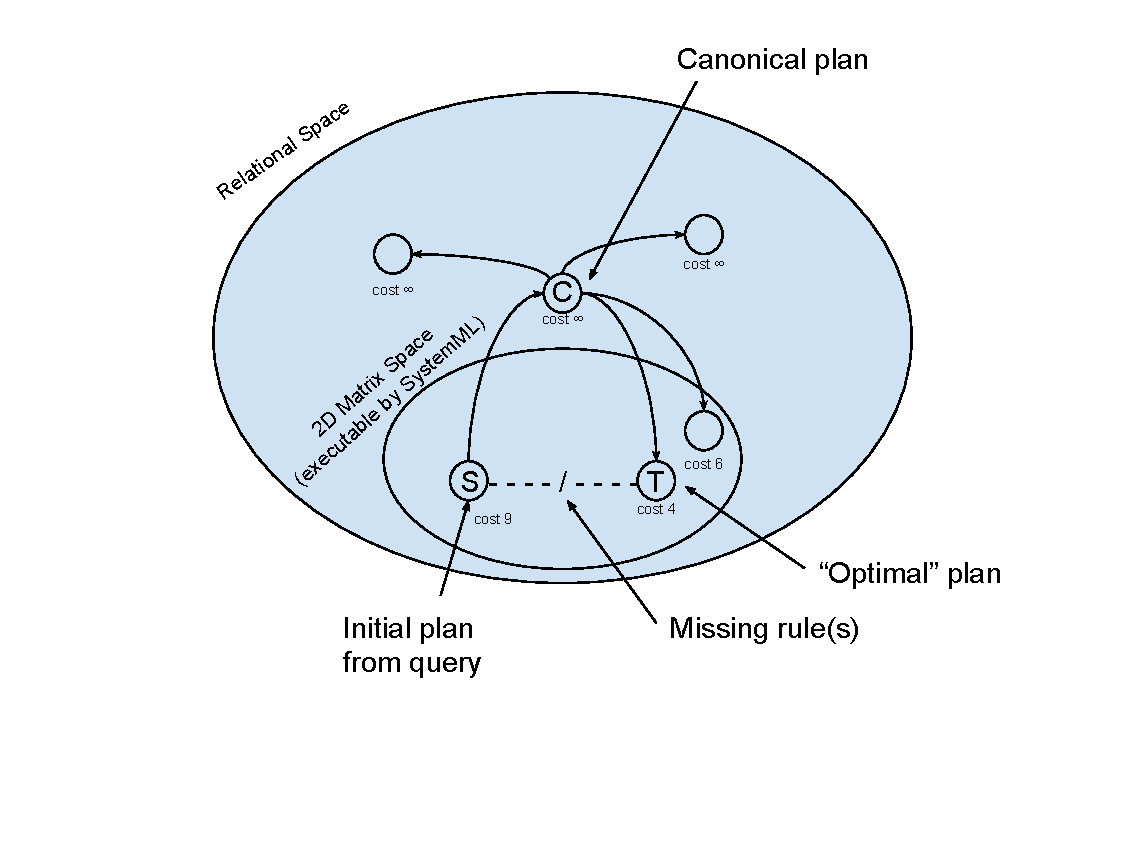
\includegraphics[trim={3cm 2cm 2cm 0},clip,width=1\linewidth]{la_to_ra_and_back}
\caption{For a given query MPlan, it is difficult to find the lowest-cost semantically equivalent MPlan due an incomplete basis: MPlan operators are compound and can be decomposed into more primitive parts. Rewriting to a canonical RPlan grants the ability to find otherwise unreachable equivalent MPlans.}
\label{fOverallPlan}
\end{figure}
\begin{figure}[tbh]
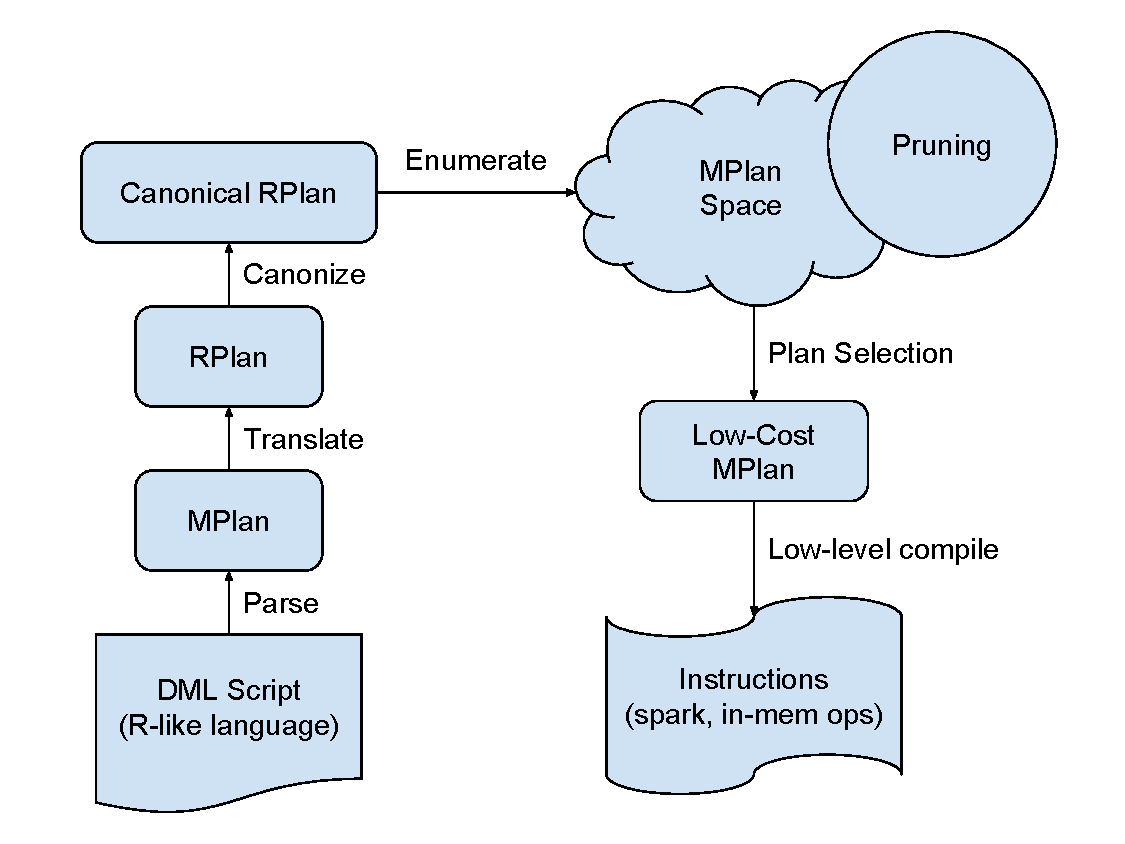
\includegraphics[trim={0 0 0 0},clip,width=1\linewidth]{la_to_ra_and_back_flowchart}
\caption{Approach to finding the lowest-cost semantically equivalent MPlan by searching through a space generated by canonical RPlans.}
\label{fOverallPlanFlowchart}
\end{figure}


\section{$ABC+BCD+ABD$}

\begin{figure*}[tbh]
\subcaptionbox{Cost in flops for a few plans computing $ABC+BCD+ABD$\label{tExCost}}{
\begin{tabular}{c|ccc}
plan & cost (dense) 
& \begin{tabular}{@{}c@{}}$n_1=2$\\$n_2=10$\end{tabular} 
& \begin{tabular}{@{}c@{}}$n_1=10$\\$n_2=2$\end{tabular} \\
\hline
$AB(C+D) + (BC)D$       & $2n_1^2 n_2 + 6n_1 n_2^2 + n_2^2 + n_1 n_2$ & 1400 & \textbf{664} \\
$(BC+AB)D + (AB)C$      & $2n_1^2 n_2 + 6n_1 n_2^2 + 2n_1 n_2$ & \textbf{1320} & 680 \\
$(AB)C + (BC)D + (AB)D$ & $2n_1^2 n_2 + 8n_1 n_2^2 + 3n_1 n_2$ & 1740 & 780 \\
$A(BC) + (BC)D + (AB)D$ & $4n_1^2 n_2 + 6n_1 n_2^2 + 3n_1 n_2$ & 1420 & 1100 \\
\end{tabular}
}
\subcaptionbox{Plot of $n_2:n_1$ ratio vs. plan cost\label{fExPlot}}{
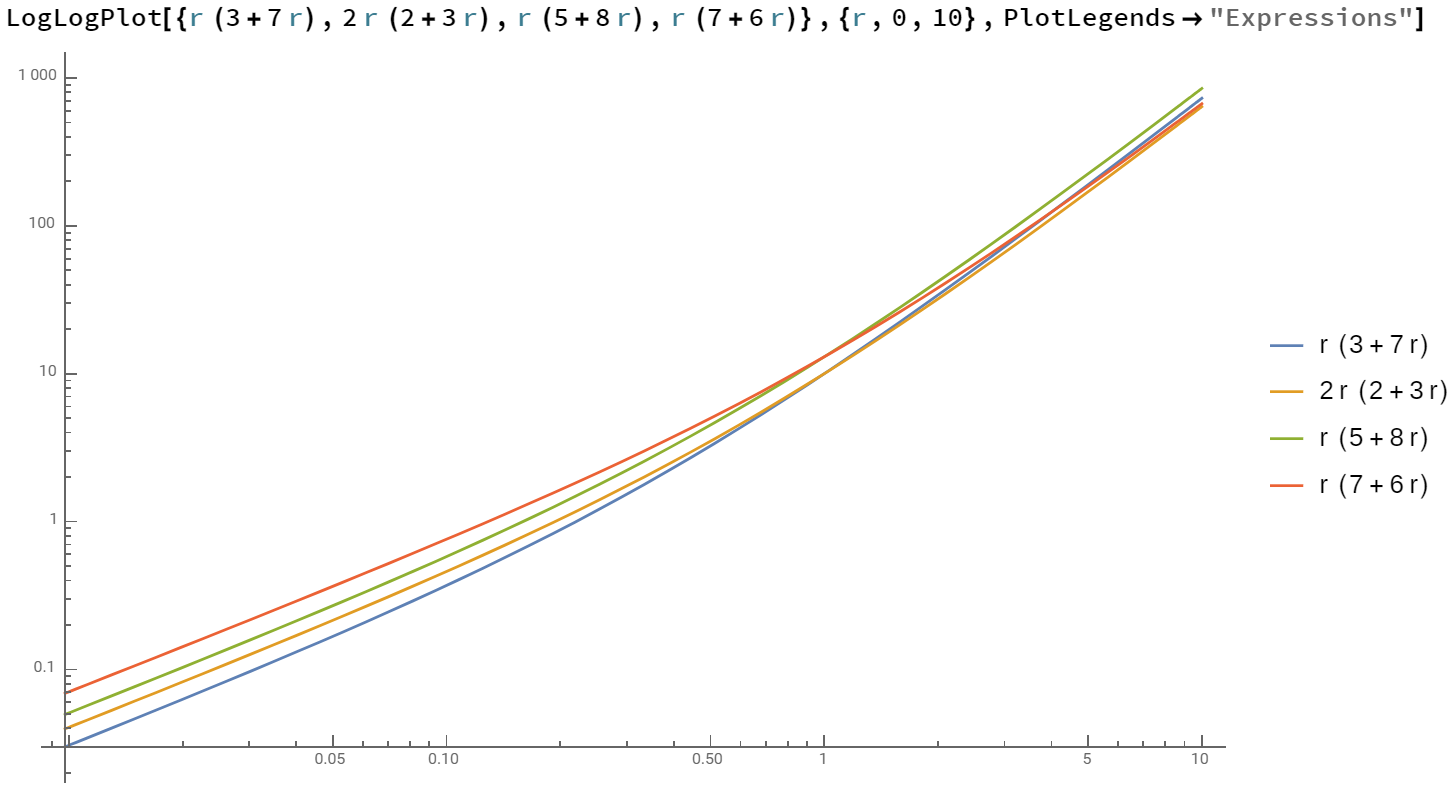
\includegraphics[width=0.32\linewidth]{ex_compare}
}
\end{figure*}

Consider the following DML program, in which $n_1$ and $n_2$ are parameters that determine the dimensions of the matrices $A$, $B$, $C$, $D$.
The \texttt{matrix} function creates dense matrices with the given dimensions, filled with the value 1.

\begin{lstlisting}[language=R,escapeinside={(*}{*)},frame=single,caption={DML Program for $ABC+BCD+ABD$},label={lExDML}]
A = matrix(1, rows=(*$n_1$*), cols=(*$n_1$*))
B = matrix(1, rows=(*$n_1$*), cols=(*$n_2$*))
C = matrix(1, rows=(*$n_2$*), cols=(*$n_2$*))
D = matrix(1, rows=(*$n_2$*), cols=(*$n_2$*))

R = A%*%B%*%C + B%*%C%*%D + A%*%B%*%D
write(R, "result.csv")
\end{lstlisting}

\subsection{Manual analysis of plans}

What is the optimal plan to compute $R$?
The answer depends on $n_1$ and $n_2$.
Table~\ref{tExCost} presents a few alternative plans that compute $R$.
The cost, in number of additions and multiplications, is given symbolically in terms of $n_1$ and $n_2$, as well as numerically with different ratios of $n_1$ and $n_2$.

Let's manually analyze the cost of a few alternative plans that compute $R$ for practice.
Recall that a dense matrix multiplication of an $a \times b$ matrix with an $b \times c$ matrix requires $ac$ inner products, each requiring $b$ multiplications and $b-1$ additions (really, $b$ additions when added to a 0 in the result matrix), for a total cost of $2abc$.

Table~\ref{tExCost} hints that the optimal plan for $R$ depends on the ratio of $n_2$ to $n_1$.
When $n_1 \ll n_2$, then the first plan appears to be cheapest. 
When $n_1 \gg n_2$, then the second plan appears to be cheapest. 
The third and fourth plans, while correct, do not appear to be cheapest for any ratio, as they do not take advantage of + factorizations.
Figure~\ref{fExPlot} on the ratio $r$ confirms this trend.

Note that the author's analysis missed a lower cost plan for inputs where $n_1 \gg n_2$.  This plan is $AB(C+D) + B(CD)$. It is easy to miss such plans during manual analysis.

A real ML program contains more complicated expressions. Manual analysis is not feasible; an automated method for finding a (near-)optimal plan is called for. Let's walk through how we could optimize this expression in a more general fashion.



\subsection{MPlans}
Different ways of representing plans can make it easier to optimize them.
One of the simplest representations is the Directed Acyclic Graph (DAG).
A DAG representation presents inputs to an expression as leaves at the bottom, outputs as roots at the top, and operators as interior nodes.

Parsers parse DML expressions into DAGs.
In our example, a parser would parse the program from Listing~\ref{lExDML} into a DAG consisting of matrix operators, shown in Figure~\ref{fExMatrixDAG}.
This parsing assumes parentheses on the left of every multiplication and addition, as in $((AB)C + (BC)D) + (AB)D$.
The order of children is significant in this representation, which we call an MPlan.

The DAG shows the common subexpression $AB$ with two parents: the node computing $ABC$ and the node computing $ABD$.
Common subexpressions are important to recognize, because they can be computed once and reused for all parents.
The process of identifying common subexpressions inside a DAG is called \textit{common subexpression elimination} (i.e., eliminating duplicate subplans by reconnecting the parents of the duplicates to a single copy of the subplan).

It is possible to optimize MPlans directly, by writing rules over the operators MxM (matrix multiplication), $*$ (element-wise multiplication), $+$ (element-wise addition), $^\tr$ (transpose), $\sum_{row}$ (row-wise aggregation), $\sum_{col}$ (column-wise aggregation), and $\sum$ (full aggregation).
However, reasoning at the matrix DAG level is prone to missing possible rewrites,
such as interchanging the $\sum$ over an MxM or $*$.
We therefore consider a finer-grained representation.

\begin{figure}[tbh]
    \centering
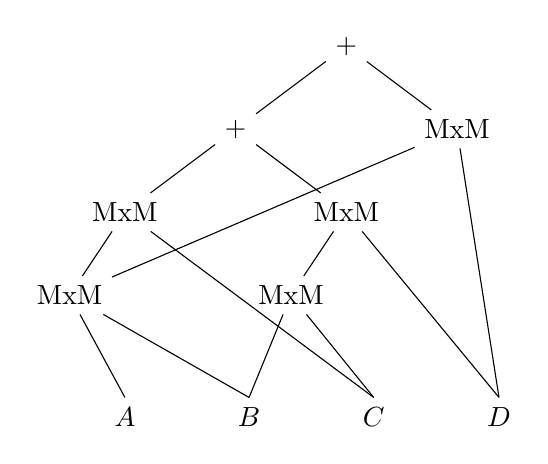
\begin{tikzpicture}[level distance=3em, node distance=3em,
    level 1/.style={sibling distance=8em},
    level 2/.style={sibling distance=8em},
    level 3/.style={sibling distance=4em},
]
\node {$+$}
    child {node {$+$}
        child {node (ABC) {MxM}
            child {node (AB) {MxM}
                % child {node (Aab) {A}} %{$B_{ae}$}
                % child {node (Bbc) {B}} %{$C_{ef}$}
            }
            child[missing]% {node (Ccd) {C}} %{$D_{fd}$}
        }
        child {node (BCD) {MxM}
            child {node (BC) {MxM}
                % child {node (Bae) {B}} %{$B_{ae}$}
                % child {node (Cef) {C}} %{$C_{ef}$}
            }
            child[missing]% {node (Dfd) {D}} %{$D_{fd}$}
        }
    }
    child {node (ABD) {MxM}
        child[missing]
        % {node {MxM}
        %     child {node (Aag) {A}} %{$A_{ag}$}
        %     child {node (Bgh) {B}} %{$B_{gh}$}
        % }
        child[missing] %{node (Dhd) {D}} %{$D_{hd}$}
    }
;
\node (A) [below=of AB,xshift=2em] {$A$};
\node (B) [right=of A] {$B$};
\node (C) [right=of B] {$C$};
\node (D) [right=of C] {$D$};

\draw (A.north) -- (AB);
% \draw (A.north) -- (Aag.south);
\draw (B.north) -- (AB);
\draw (B.north) -- (BC);
% \draw (B.north) -- (Bgh.south);
\draw (AB) -- (ABD);
\draw (C.north) -- (ABC);
\draw (C.north) -- (BC);
\draw (D.north) -- (BCD);
\draw (D.north) -- (ABD);
\end{tikzpicture}
    \caption{MPlan, parsed from Listing~\ref{lExDML}}
    \label{fExMatrixDAG}
\end{figure}



As a brief note, we would like to mention that DML programs contain compound operators in addition to the ones listed above.
For example, $-$ (element-wise subtraction) and \^{} (element-wise power) are DML operators that can be written in terms of more basic ones, by applying the rules
\begin{align*}
A - B &\to A + (-1)*B \\
\forall k \in \textsc{Z}^+,\, A^k &\to A * A^{k-1} \\
A^0 &\to 1
\end{align*}

Other operators in DML, such as min and max, cbind (horizontal concatenation), reshape (permute the entries of a matrix into a different shape), and table (construct a matrix from a vector of row indices, a vector of column indices, and a vector of values) are deferred to future work. Including these operators is important because it may be possible to optimize through them by, for example, pushing down a matrix multiply through a cbind($A$,$B$) operator in order to optimize it with the plans that compute $A$ and $B$. In this work, we simply model these operators as uninterpreted black boxes.



\subsection{RPlan DAG}
The elementary operators of linear algebra are patterns of $+$ and $*$.
In this section we introduce two patterns that have sufficient expressiveness to represent all the matrix operators in the MPlans.  We call the new representation RPlans, short for relation plans.

The first pattern is the join.  
Element-wise addition or multiplication join their arguments on matching row and column indices, adding or multiplying matching values.
The first stage of matrix multiply joins the column indices of the first matrix to equal row indices of the second matrix, multiplying matching values.
The first stage of the inner product of two vectors joins on their matching indices.
The outer product of two vectors joins without any join conditions, i.e., taking the Cartesian product of indices.
Thus, joins in linear algebra may involve 0, 1, or 2 join conditions of indices.

In the spirit of relational algebra, from which we borrow the join operation, we will refer to indices as \textit{attributes}.
The objects in the RPlan algebra representation can be considered \textit{relations},
whose attribute names are known as its \textit{schema}.
The schema of a join has attributes equal to the union of its inputs' schema.

We use the symbols $*$ and $+$ to denote the $n$-ary join that multiplies or adds matching values.
The two operators are similar, but there is an important difference between them.  
If we imagine the value 0 as a ``null value'' in the relational sense,
then $*$ acts like an inner join, because multiplication has the annihilator property that for any number $x$, $0 * x = 0$,
whereas $+$ acts like an outer join, because addition does not have the annihilator property.
Nuances like these are important when writing a cost model.
%k-relation

In order to represent join conditions, we adopt the convention of natural join semantics, i.e., that attributes whose names match are meant to be joined together.
We use two operators to manage attributes:
the \textit{bind} operator to assign attribute names, and the \textit{unbind} operator to un-assign attributes.
We write $\bind{ab}$ to bind the indices $a$ and $b$ to the rows and columns of a matrix.
We write $\unbind{ab}$ to un-assign the attribute $a$ as the row and $b$ as the column in a matrix.
Vectors require only one attribute name, because they have a single dimension.

The semantics of bind are to open a stream of scalars from the input that are labelled with the attribute names they are bound to.  Bound names may be thought of as iterating over the input values.
The semantics of unbind are to collect a stream of scalars into a matrix object, using the positions of the unbound attributes to determine which index is the row and which is the column.

The transpose operator is therefore represented in RPlans as an unbind that reverses the order of unbound names.
For example, the plan $\unbind{ba}( \bind{ab}A )$ transposes the input $A$ by unbinding index names opposite the order in which the indices were bound.

Applying this to matrix multiply, the first stage of the plan $A \text{ MxM } B$ can be represented as $\bind{ab} A * \bind{bc} B$.
The name $b$ joins the rows of $A$ to the columns of $B$.  
The result is a 3-tensor, i.e. a tensor of 3 dimensions, because it has three attributes in its schema: $a, b, c$.

The final part of a matrix multiply can be represented with aggregation over $b$.
Aggregation is an operator that is annotated with the attributes to be aggregated, in this case $\sum_b$.
The schema of an aggregation is the schema of its input minus the aggregated attributes.
Thus, a complete expression for the plan $A \text{ MxM } B$ is $\unbind{ac} \sum_b( \bind{ab} A * \bind{bc} B )$.








\subsection{RPlan DAG in Canonical Form}
A common way to write the example in math, assuming parentheses on the left of every multiplication, is
\begin{align*}
R_{ad} &= 
\sum_c \lrparen{\sum_b A_{ab} B_{bc}} C_{cd} + 
\sum_f \lrparen{\sum_e B_{ae} C_{ef}} D_{fd} \\&\qquad\qquad +
\sum_h \lrparen{\sum_g A_{ag} B_{gh}} D_{hd} \\
&= \sum_{bc} A_{ab} B_{bc} C_{cd} + \sum_{ef} B_{ae} C_{ef} D_{fd} + \sum_{gh} A_{ag} B_{gh} D_{hd}
\end{align*}
The above math includes indices (i.e., the letters $a, b, c$, etc.) that bind to the rows and columns of the input matrices, in a way that matches the semantics of matrix multiplication:
the column of the first matrix joins to (has the same attribute name as) the row of the second matrix, which is aggregated away after multiplication.
The rewriting uses the distributive law of $*$ over $\sum$ and the commutativity of $\sum$ to pull the aggregation operators to the top of the expression and push the multiplication operators to the bottom.  

% Talk about relational interpretation over k-relations? 

``Top'' and ``bottom'' refer to the presentation of the expression in the form of a DAG.  
The DAG has one root corresponding to the output of the expression, and one leaf for each input. 
Internal nodes take the form of $+$, $*$, and $\sum$.
Figure \ref{fExDag} presents a DAG of the expressions both before and after rewriting into canonical form.

In general, the canonical form of an RPlan is one that, from bottom to top, includes the inputs, a bind layer, a multiplication layer, an aggregation layer, an addition layer, and an unbind layer.

\begin{figure}[tbh]
    \centering
\subcaptionbox{Plan to compute $((AB)C+(BC)D)+(AB)D$\label{fExDagOrig}}{
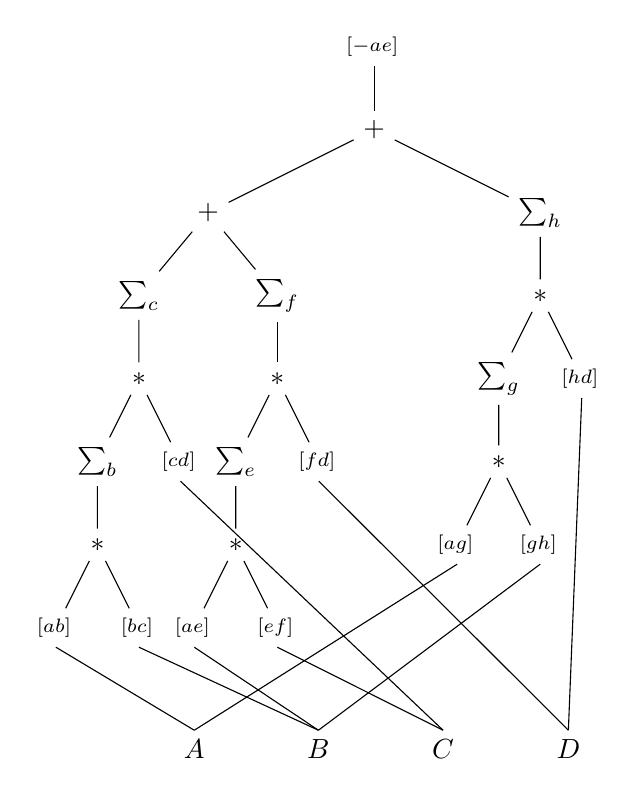
\begin{tikzpicture}[level distance=3em, node distance=3em,
    level 2/.style={sibling distance=12em},
    level 3/.style={sibling distance=5em},
    level 4/.style={sibling distance=3em},
]
\node {\unbind{ae}}
child {node {$+$}
    child {node {$+$}
        child {node {$\sum_{c}$} child {node {$*$}
            child {node {$\sum_b$} child {node {$*$}
                child {node (Aab) {\bind{ab}}} %{$B_{ae}$}
                child {node (Bbc) {\bind{bc}}} %{$C_{ef}$}
            }}
            child {node (Ccd) {\bind{cd}}} %{$D_{fd}$}
        }}
        child {node {$\sum_{f}$} child {node {$*$}
            child {node {$\sum_e$} child {node {$*$}
                child {node (Bae) {\bind{ae}}} %{$B_{ae}$}
                child {node (Cef) {\bind{ef}}} %{$C_{ef}$}
            }}
            child {node (Dfd) {\bind{fd}}} %{$D_{fd}$}
        }}
    }
    child {node {$\sum_{h}$} child {node {$*$}
        child {node {$\sum_g$} child {node {$*$}
            child {node (Aag) {\bind{ag}}} %{$A_{ag}$}
            child {node (Bgh) {\bind{gh}}} %{$B_{gh}$}
        }}
        child {node (Dhd) {\bind{hd}}} %{$D_{hd}$}
    }}
};
\node (A) [below=of Bbc,xshift=2em] {$A$};
\node (B) [right=of A] {$B$};
\node (C) [right=of B] {$C$};
\node (D) [right=of C] {$D$};

\draw (A.north) -- (Aab.south);
\draw (A.north) -- (Aag.south);
\draw (B.north) -- (Bbc.south);
\draw (B.north) -- (Bae.south);
\draw (B.north) -- (Bgh.south);
\draw (C.north) -- (Ccd.south);
\draw (C.north) -- (Cef.south);
\draw (D.north) -- (Dfd.south);
\draw (D.north) -- (Dhd.south);
\end{tikzpicture}
}

\subcaptionbox{Plan rewritten into canonical form\label{fExDagCanonical}}{
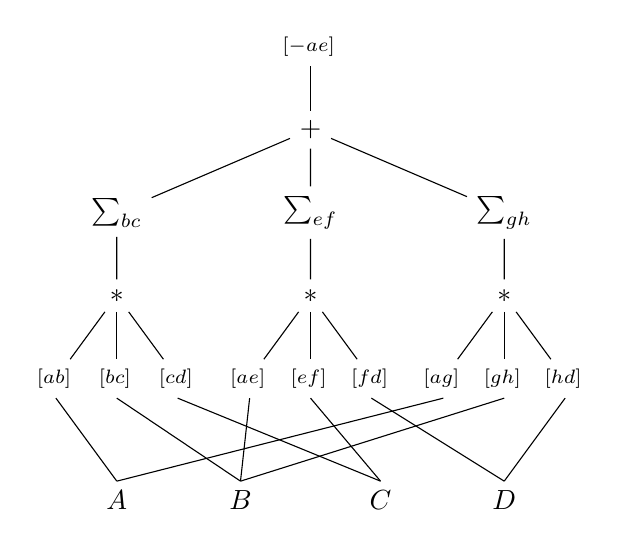
\begin{tikzpicture}[level distance=3em, node distance=3em,
    level 2/.style={sibling distance=7em},
    level 3/.style={sibling distance=3.5em},
    level 4/.style={sibling distance=2.2em},
]
\centering
\node {\unbind{ae}}
child {node {$+$}
    child {node {$\sum_{bc}$}
        child {node {$*$}
            child {node (Aab) {$\bind{ab}$}} %{$A_{ab}$}
            child {node (Bbc) {\bind{bc}}} %{$B_{bc}$}
            child {node (Ccd) {\bind{cd}}} %{$C_{cd}$}
        }
    }
    child {node {$\sum_{ef}$}
        child {node {$*$}
            child {node (Bae) {\bind{ae}}} %{$B_{ae}$}
            child {node (Cef) {\bind{ef}}} %{$C_{ef}$}
            child {node (Dfd) {\bind{fd}}} %{$D_{fd}$}
        }
    }
    child {node {$\sum_{gh}$}
        child {node {$*$}
            child {node (Aag) {\bind{ag}}} %{$A_{ag}$}
            child {node (Bgh) {\bind{gh}}} %{$B_{gh}$}
            child {node (Dhd) {\bind{hd}}} %{$D_{hd}$}
        }
    }
};
\node (A) [below=of Bbc] {$A$};
\node (B) [below=of Bae,xshift=-.33em] {$B$};
\node (C) [below=of Dfd,xshift=.33em] {$C$};
\node (D) [below=of Bgh] {$D$};

\draw (A.north) -- (Aab.south);
\draw (A.north) -- (Aag.south);
\draw (B.north) -- (Bbc.south);
\draw (B.north) -- (Bae.south);
\draw (B.north) -- (Bgh.south);
\draw (C.north) -- (Ccd.south);
\draw (C.north) -- (Cef.south);
\draw (D.north) -- (Dfd.south);
\draw (D.north) -- (Dhd.south);
\end{tikzpicture}
}
    \caption{DAG representation of plans to compute $ABC+BCD+ABD$}
    \label{fExDag}
\end{figure}



\subsection{Mockup bottom-up plan search}





\section{Formal Definitions}

\subsection{MPlans, RPlans, Mixed Plans}

\begin{table}[tbh]
\begin{tabular}{llll}
&name & type & syntax \\
\hline
\multirow{7}{*}{\rotatebox[origin=c]{90}{MPlan}} 
&mmult & $M_{M,L} \times M_{L,N} \rightarrow M_{M,N}$ & $AB$ or MxM \\
&elemmult & $M_{M,N} \times M_{M,N} \rightarrow M_{M,N}$ & $A*B$ \\
&elemplus & $M_{M,N} \times M_{M,N} \rightarrow M_{M,N}$ & $A+B$ \\
&rowagg & $M_{M,N} \rightarrow M_{M,1}$ & $\sum_{row} A$ \\
&colagg & $M_{M,N} \rightarrow M_{1,N}$  & $\sum_{col} A$ \\
&agg & $M_{M,N} \rightarrow M_{1,1}$ & $\sum A$ \\
%&power & $M  \times Int \rightarrow M$ & $A^k$ \\
&transpose & $M_{M,N} \rightarrow M_{N,M}$ & $A^\tr$ \\
\hline
\multirow{2}{*}{\rotatebox[origin=c]{90}{conv.}}
&bind & $M_{M,N} \times [i,j] \rightarrow R_{i:M,j:N}$ & $\bind{i,j} A$ \\
&unbind & $R_{i:M,j:N} \times [i,j] \rightarrow M_{M,N}$ & $\unbind{i,j} A$ \\
\hline
\multirow{2}{*}{\rotatebox[origin=c]{90}{RPlan}}
&join & $R_{S_1} \times R_{S_2} \rightarrow R_{S_1 \cup S_2}$ & $A*B$ or $A+B$ \\
&agg & $R_S \times U \rightarrow R_{S \setminus U}$ & $\sum_{U} A$ \\
\end{tabular}
\caption{Operators of MPlans and RPlans. Uninterpreted black-box functions are also allowed.
The type $M_{M,N}$ is a matrix of size $M \times N$; $[i,j]$ is a list of attribute names; $R_{i:M,j:N}$ is a relation with attributes $i$ of size $M$ and $j$ of size $N$; $S_1, S_2, S,$ and $U$ are sets of attributes.}
\label{tPlanOps}
\end{table}

The Matrix Plan Algebra is an algebra over real number matrices with the operators listed in the top third of Table~\ref{tPlanOps}. 
The type of an matrix with dimensions $M \times N$ is written $M_{M,N}$.
Vectors have orientation and are written as either $M_{1,N}$ or $M_{M,1}$; scalars have type $M_{1,1}$.
An \textit{MPlan}---short for Matrix Plan---is an expression in the Matrix Plan Algebra. 

The Relation Plan Algebra is an algebra over relations (whose attributes' domain is a prefix of the positive integers) with the operators listed in the bottom third of Table~\ref{tPlanOps}.
The domain of each attribute is a prefix of the positive integers; we say an attribute has size $s$ if its domain is the integers $1, 2, \dots, s$.
The notation $R_{i:M,j:N,k:L}$ indicates a relation $R$ with attributes $i$ of size $M$, $j$ of size $N$, and $k$ of size $L$.
Each tuple of a relation is annotated with a real number.
The set of a relation's attributes is called its schema.
We write $i \in A$ if $i$ is an attribute name present in $A$'s schema.
An \textit{RPlan}---short for Relation Plan---is an expression in the Relation Plan Algebra.

The middle third of Table~\ref{tPlanOps} presents the bind and unbind conversion operators between matrices and relations. Both operators are annotated with a pair of attribute names, either of which may be the `\_' symbol to match the dimension of the input type. % whose length matches the input's dimension 

\begin{definition}
An \textbf{\emph{MPlan}} is an expression in the Matrix Plan Algebra, except that relation objects (but not relation operators) and conversion operators are also allowed. An MPlan is \emph{pure} if it does not contain conversion operators.

An \textbf{\emph{RPlan}} is an expression in the Relation Plan Algebra, except that matrix objects (but not matrix operators) and conversion operators are also allowed. An RPlan is \emph{pure} if it does not contain conversion operators.

A \textbf{\emph{Mixed Plan}} is an expression in the product of the Matrix Plan Algebra and the Relation Plan Algebra, extended with the conversion operators.
\end{definition}

MPlans, RPlans, and Mixed Plans are depicted as DAGs, to emphasize that they may contain common sub-expressions (CSEs) or multiple outputs (multiple roots).
They may also contain uninterpreted (black-box) functions.



\subsection{Converting MPlans to RPlans}
An MPlan may be converted into a semantically equivalent RPlan via the rewrite rules $R_{MR}$ in Figure~\ref{RMR}.
This list includes additional rules for a couple common operators in the DML language: element-wise subtraction and positive integer exponentiation.

\begin{figure}[htb]
\begin{enumerate}
  \item $A - B \rightarrow A + (-1) * B$
  \item For small integers $k > 1$, $A^k \rightarrow A * A^{k-1}$ and $A^1 \to A$.
  \item $A*B \rightarrow \unbind{i,j}(\bind{i,j}A * \bind{i,j}B)$.  Same pattern for $+$.
  \item $AB \rightarrow \unbind{i,k} \sum_j (\bind{i,j}A * \bind{j,k}B)$. 
  \item $A^\tr \rightarrow \unbind{j,i} \bind{i,j}A$.
  \item $\sum_{row} A \rightarrow \unbind{i,\_} \sum_j \bind{i,j} A$.  Similar pattern for $\sum_{col}$, $\sum$.
\end{enumerate}
\caption{MPlan-to-RPlan Ruleset $R_{MR}$}
\label{RMR}
\end{figure}

Applying the $R_{MR}$ rules replaces matrix operators with relation operators, with conversion operators in between to convert matrices to relations and back. The result is an RPlan.

It follows from the $R_{MR}$ rules that the space of MPlans is a subset of the space of RPlans. We prove that it is a strict subset in the following:
\begin{lemma}
Let \MPLAN{} and \RPLAN{} be the set of all MPlans and RPlans.
Then $R_{MR}(\MPLAN{}) \subsetneq \RPLAN{}$.
\end{lemma}

% No confluence needed (confluence means that no matter what order we apply RMR rules, the result is the same).

\begin{proof}
First we need to show that the ruleset $R_{MR}$ is terminating on any MPlan, or else the lemma is improper. It is terminating because each rule (except (1)) removes a matrix operator, and an MPlan has finitely many matrix operators. For rule (2), we use the fact that $k$ decreases and is bounded below to prove termination.

Suppose $p \in \MPLAN{}$. 
We prove that $R_{MR}(p) \in \RPLAN{}$ by structural induction on $p$. 
The base case, that $p$ is a lone matrix, is trivially an RPlan.
The rules $R_{MR}$ compose the inductive case; for each matrix operator, there is a rule in $R_{MR}$ that converts it to a composition of relation operators and conversion operators.  Rule (2) requires a second induction, but otherwise the proof is straightforward. 

To show that $R_{MR}(\MPLAN{}) \neq \RPLAN{}$, consider the RPlan $\bind{i,j}A * \bind{k,l}B$.
This RPlan computes a tensor product and has schema $\{i,j,k,l\}$. As its dimension is 4, no representation as an MPlan is possible because the maximum dimension of an MPlan is 2.
\end{proof}


The unbind and bind operators can be eliminated or moved around to create ``pipelines'' of RPlan operators.
For example, the rule $\bind{i,j} \unbind{i,j} A \to A$ removes a bind-unbind sequence, assuming that care is taken to properly handle CSEs.
More generally the rule $\bind{x,y} \unbind{i,j} A \to A[i \to x, j \to y]$ indicates that the attributes $i$ and $j$ in $A$'s schema should be renamed to $x$ and $y$, by propagating the rename downward into $A$.
%This pattern will be discussed in more detail.
The result of eliminating/shifting unbind and bind operators is an RPlan with a bind operator above every (nonscalar) input and an unbind operator below every (nonscalar) output.


\subsection{RPlan Canonical Form}
We now introduce a canonical form for RPlans.
The purpose of the form is to (1) identify common sub-expressions (i.e., expressions that may differ in syntax but compute the same function) and (2) act as a neutral starting point from which we may systematically enumerate alternative plans.  Fulfilling these roles requires the canonical property, that two RPlans have the same canonical form if and only if they are semantically equivalent (i.e., they compute the same result on every input).%\footnote{Our canonical form technically is only canonical up to uninterpreted constants. Constant folding, such as replacing $2 + 3$ with 5, occurs before and after our optimization process and affects the estimated cost of plans little.}

Our form is similar in spirit to the disjunctive normal form (DNF) in propositional logic, also known as a truth table.  DNF formulae are rarely the most efficient form to execute, but they do act as a canonical form and also serve as a starting point for finding more efficient forms.  %((Reference K-V maps?))
Our form is also similar to the canonical form of polynomials as a sum of monomials, except that the monomial terms also include aggregations and constants are treated as black-box symbols, rather than real numbers.

The analogy to polynomials extends further: the canonical form of polynomials combines ``like terms,'' i.e., two terms that have the same variables.  Instead of writing $3x^2y + 5x^2y$, for example, we write its canonical form as $8x^2y$.
For RPlans, we determine whether two terms are like by whether there exists an isomorphism mapping one to the other by renaming attributes (up to a constant scalar).

The canonical form for MPlans is the sum-of-aggregations-of-products with like terms combined, as follows:

\begin{definition}
An RPlan is \textbf{canonical} if it can be written as the sum of $n$ terms, each of which is an aggregation over a (possibly empty) attribute set $A_i$ (for $1 \leq i \leq n$), each of whose inputs is the multiplication of $m_i$ base input matrices $b_{ij}$ (for $1 \leq i \leq n$, $1 \leq j \leq m_i$):

\[\sum_{A_1} \lrparen{b_{11} * \dots * b_{1m_1}} %+ \sum_{A_2} (b_{21} * \dots * b_{2m_2})
+ \dots + \sum_{A_n} \lrparen{b_{n1} * \dots * b_{nm_n}}\]

Further, there must not exist, for any $1 \leq i < j \leq n$, an isomorphism $\phi$ renaming attributes in the schema of $b_{i1} * \dots * b_{im_i}$ to attributes in the schema of $b_{j1} * \dots * b_{jm_j}$ such that $m_i=m_j$, $\phi(A_i) = A_j$, and $\phi\{b_{i1} * \dots * b_{im_i}\} = \{b_{j1} * \dots * b_{jm_j}\}$.

The order of summands and multiplicands is insignificant, due to the commutative and associative properties of $*$ and $+$. A canonical order within these can be established when necessary by, e.g., hashing.

% A canonical form may be abbreviated as \\
% $[(A_1; b_{11}, \dots, b_{1m_1}), \dots, (A_n; b_{n1}, \dots, b_{nm_n})]$.
\end{definition}

Figure~\ref{RRC} shows the rewrite rules $R_{RC}$ that canonize RPlans by pulling additions to the top of an expression, followed by aggregations and last multiplications. 
Let $\mathcal{C}$ be the transitive application of ruleset $R_{RC}$.

\begin{figure}[htb]
\begin{enumerate}
  \item\label{RRC_mp} $A * (B + C) \rightarrow A*B + A*C$
  \item\label{RRC_ap} $\sum_i (A + B) \rightarrow \sum_i A + \sum_i B$
  \item\label{RRC_ma} If $i \not\in A$,  $A * \sum_i B \rightarrow \sum_i (A * B) \quad$ (else rename indices)
  \item\label{RRC_aa} $\sum_i \sum_j A \rightarrow \sum_{i,j} A$
%   \item $\sum_i A \rightarrow \sum_{i,j} A$
  \item\label{RRC_ac} If $i \not\in A$, then $\sum_i A \rightarrow A * |i|$
  \item\label{RRC_pp} $A + (B + C) \rightarrow +(A, B, C) \quad$ (binary to n-ary addition)
  \item\label{RRC_mm} $A * (B * C) \rightarrow *(A, B, C) \quad$ (binary to n-ary multiply)
  \item\label{RRC_c} Constant fold constant terms $c_1 + c_2$, $c_1*c_2$
  \item\label{RRC_cc} 
  If $c_1, c_2$ are constant and $T_1, T_2$ are isomorphic up to renaming,
  then $c_1 * T_1 + c_2 * T_2 \to (c_1 + c_2) * T_1$ and apply rule (\ref{RRC_c})
\end{enumerate}
\caption{RPlan-to-Canonical-RPlan Ruleset $R_{RC}$}
\label{RRC}
\end{figure}

We now prove a few properties of $\mathcal{C}$ in order to show that it truly is canonizing.
% Each rewrite preserves the expression's semantics, as they stem from the mathematics of semirings and aggregates.

\begin{lemma}
$\forall p \in \RPLAN{},\, \mathcal{C}(p)$ is in canonical form. 
\end{lemma}
\begin{proof}
$R_{RC}$ rules 8 and 9 combine isomorphic-up-to-constant terms.

Proceed by structural induction over an RPlan $p$.
The base case, that $p$ is a lone relation, is canonical.
The inductive cases are as follows.

1) Suppose $p = p^1 + p^2$. 
By the inductive hypothesis, $p^1$ and $p^2$ are canonical with forms, for $i \in \{1,2\}$, \\ 
$\sum_{A^i_{1}} \lrparen{b^i_{11} * \dots * b^i_{1m^i_{1}}} + \dots + \sum_{A^i_{n^i}} \lrparen{b^i_{n^i1} * \dots * b^i_{n^im^i_{n^i}}}$.

By rule~\ref{RRC_pp}, $p$ takes the canonical form \\
$\sum_{A^1_{1}} \lrparen{b^1_{11} * \dots * b^1_{1m^1_{1}}} + \dots + \sum{A^1_{n^1}} \lrparen{b^1_{n^11} * \dots * b^1_{n^1m^1_{n^1}}} +
\sum_{A^2_{1}} \lrparen{b^2_{11} * \dots * b^2_{1m^2_{1}}} + \dots + \sum{A^2_{n^2}} \lrparen{b^2_{n^21} * \dots * b^2_{n^2m^2_{n^2}}}$.

2) Suppose $p = \sum_A p'$.
By the inductive hypothesis, $p'$ is canonical with form \\
$\sum_{A_1} \lrparen{b_{11} * \dots * b_{1m_1}} + \dots + \sum_{A_n} \lrparen{b_{n1} * \dots * b_{nm_n}}$.

Rule \ref{RRC_ap} distributes the aggregate into plus;
rule \ref{RRC_ac} handles constant aggregations, as after the expression $\sum_{ij} (X + 7)$;
rule \ref{RRC_aa} combines aggregates.
The result has canonical form \\
$\sum_{A_1 \cup A} \lrparen{b_{11} * \dots * b_{1m_1}} + \dots + \sum_{A_n \cup A} \lrparen{b_{n1} * \dots * b_{nm_n}}$.

3) Suppose $p = p^1 * p^2$.
By the inductive hypothesis, $p^1$ and $p^2$ are canonical with forms, for $i \in \{1,2\}$, \\ 
$\sum_{A^i_{1}} \lrparen{b^i_{11} * \dots * b^i_{1m^i_{1}}} + \dots + \sum_{A^i_{n^i}} \lrparen{b^i_{n^i1} * \dots * b^i_{n^im^i_{n^i}}}$.
% $\sum_{A_{i1}} \lrparen{b_{i11} * \dots * b_{i1m_1}} + \dots + \sum{A_{in}} \lrparen{b_{in1} * \dots * b_{inm_n}}$.

Rule \ref{RRC_mp} multiplies across the Cartesian product of summands of $p_1$ and $p_2$.
Rules \ref{RRC_ma}, \ref{RRC_mm}, and \ref{RRC_aa} push the multiplications further down into aggregations and other multiplications.
In particular, rule \ref{RRC_ma} may rename attributes; we use the `$\sqcup$' symbol to denote disjoint union after renaming.
The result is the canonical form \\
$\sum_{A^1_{1} \sqcup A^2_{1}} \lrparen{b^1_{11} * \dots * b^1_{1m^1_1} * b^2_{11} * \dots * b^2_{1m^2_1}} + \dots + \\
\sum_{A^1_{n^1} \sqcup A^2_{n^2}} \lrparen{b^1_{n^11} * \dots * b^1_{n^1m^1_{n^1}} * b^2_{n^21} * \dots * b^2_{n^2m^2_{n^2}}}$.
\end{proof}


\begin{lemma}\label{lCanonPreservesSemantics}
Canonization preserves semantics: \\
$\forall p \in \RPLAN{}, \forall \text{inputs } d,\, p(d) = \mathcal{C}(p)(d)$.
\end{lemma}
\begin{proof}
Every rule composing $\mathcal{C}$ in $R_{RC}$ stems from a mathematical property of $+$, $*$, and $\sum$.
\end{proof}

In the following proof, we write syntactic equality with the symbol $\equiv$, in order to distinguish it from value equality.

\begin{theorem}
Two RPlans are semantically equivalent iff they have identical canonical forms:
$\forall p_1, p_2 \in \RPLAN{},\, \mathcal{C}(p_1) \equiv \mathcal{C}(p_2) \iff \forall \text{inputs }d,\, p_1(d) = p_2(d)$.
\end{theorem}
\begin{proof}
For the $\Rightarrow$ direction, two plans that have syntactically identical canonical forms must compute the same result on every input because, per Lemma \ref{lCanonPreservesSemantics}, canonization preserves semantics.

The $\Leftarrow$ direction is more interesting. Proceed by proving its contrapositive:
$\mathcal{C}(p_1) \not\equiv \mathcal{C}(p_2) \Rightarrow \exists d,\, p_1(d) \neq p_2(d)$.

It is sufficient to prove 
$\mathcal{C}(p_1) \not\equiv \mathcal{C}(p_2) \Rightarrow \exists d,\, \mathcal{C}(p_1)(d) \neq \mathcal{C}(p_2)(d)$
because, by Lemma \ref{lCanonPreservesSemantics}, $\mathcal{C}(p)(d) = p(d)$.

To find a $d$ that the canonical forms disagree on, given that the canonical forms syntactically differ,
we supply a partial input (i.e., input relations with holes) that reduces each $\mathcal{C}(p)$ to syntactically different polynomials in canonical form.
Then, by Lemma XX, we use the fact that syntactically different polynomials in canonical form differ on a concrete input, 
and we construct a full input database $d$ using this concrete input to finish the proof.

First we construct a partial input.
Pick a term $t_0 \in p_1$ such that $t_0 \not\in p_2$. Such a term must exist because $p_1 \not\equiv p_2$. [Todo: introduce graphs]
Next pick the term $t \in p_1 \text{ or } p_2$ such that $t$ is the maximal term among all terms in $p_1$ and $p_2$ that have a surjective homomorphism to $t$.

We shall design a partial input database using $t$.
Suppose there are $n$ attributes (before aggregating) in $t$.
Assign each attribute a unique positive integer between $1$ and $n$ and let $g$ be the bijection from $t$'s attributes to $[n]$.

For each multiplicand $A_{ij}$, introduce a fresh scalar variable $a_{ij}$ at entry $(g(i), g(j))$ of the input matrix $A$.
Let other entries in each input matrix be 0.

Expand the aggregations in $p_1$ and $p_2$ with respect to the new symbolic matrices.
The result is a polynomial in canonical form.
It is in canonical form because the sums-of-aggregations-of-products in the original RPlans expands to a polynomial in sum-of-products form,
and as no two terms in the original RPlan were isomorphic, neither are any two terms in the polynomial. Todo: say more about the surjective homomorphism.

Call the above reduction $d(t)$, where $t$ is the term chosen by the above process. We write $t_1[d(t)]$ for the result of applying the partial input generated by term $t$ to $t_1$. Two properties of the transformation are relevant:
\begin{enumerate}
    \item For any two terms $t_1$ and $t_2$ that are isomorphic, $t_1[d(t)] \equiv t_2[d(t)]$.
    To see this, observe that each multiplicand in $t_1[d(t)]$ arose from a multiplicand in $t_1$, and that there is an equivalent multiplicand in $t_2[d(t)]$ multiplied in the same way due to the isomorphism between $t_1$ and $t_2$.
    \item For any terms $t_1$ and $t_2$ that are not isomorphic, if there does not exist a surjective homomorphism from $t_2$ to $t_1$, then $t_1[d(t)] \not\equiv t_2[d(t)]$. Proof todo.
\end{enumerate}

Because $\mathcal{C}(p_1)$ syntactically differs from $\mathcal{C}(p_2)$, then by the second property above it follows that $\mathcal{C}(p_1)[d(t)]$ is a polynomial that syntactically differs from $\mathcal{C}(p_2)[d(t)]$.
Applying Lemma XX on polynomial canonical forms proves that a particular input on the polynomial variables $d$ exists on which the two polynomials disagree.  Plugging $d$ into the symbolic matrices designed by $d(t)$ results in a database input to the original RPlans disagree, showing that $\exists d,\, \mathcal{C}(p_1)(d) \neq \mathcal{C}(p_2)(d)$.
\end{proof}




\subsection{RPlan Graphbag}
% An RPlan \textit{without uninterpreted functions}\footnote{Uninterpreted functions split an RPlan in two: the RPlan below and the RPlan above. Each may be represented as a separate RPlan Graphbag.} in canonical form may be represented as a bag of hypergraphs, defined as follows.
% Each child of $+$ is represented as a separate graph, the collection of which forms a bag of graphs.
% A child of $+$ consists of a set of aggregated attributes, followed by the product of inputs.
% The graph is a directed and labeled hypergraph.
% The vertices $V$ are the union of the schemas of the inputs.
% Each vertex is either \textit{aggregated}, if it is in the set of aggregated attributes, or \textit{output}, if it is not.
% There is one hyperedge for each input, labeled with the input itself, on the vertices in its schema *** todo need to include the input bind and output bind *** redefine to include conv. operators -- RPlan+




\nocite{CohenDDHW09}


% OLD VERSION
% For the $\Rightarrow$ direction, two plans that have syntactically identical canonical forms must compute the same result on every input because, per Lemma \ref{lCanonPreservesSemantics}, canonization preserves semantics.

% The $\Leftarrow$ direction is more interesting. Proceed by proving its contrapositive:
% $\mathcal{C}(p_1) \neq_{syn} \mathcal{C}(p_2) \Rightarrow \exists d,\, p_1(d) \neq p_2(d)$.

% It is sufficient to prove 
% $\mathcal{C}(p_1) \neq_{syn} \mathcal{C}(p_2) \Rightarrow \exists d,\, \mathcal{C}(p_1)(d) \neq \mathcal{C}(p_2)(d)$
% because, by Lemma \ref{lCanonPreservesSemantics}, $\mathcal{C}(p)(d) = p(d)$.

% To find a $d$ that the canonical forms disagree on, 
% given that the canonical forms syntactically differ, 
% we use derivatives.  
% It is well known that for any differentiable functions $f$ and $g$, $\forall d,\, f(d) = g(d) \Rightarrow \forall d,\, f'(d) = g'(d)$; the contrapositive of this fact gives us the proof technique we need.

% In order to take derivatives, we intentionally blur the line between RPlans and (multi)linear algebra, because an RPlan relation with $n$ attributes is equivalent to a tensor with $n$ named dimensions.

% Let $t$ be one of the summed terms in $\mathcal{C}(p_1)$ that does not appear in $\mathcal{C}(p_2)$, which must exist since they syntactically differ.
% By definition of the canonical form, no other term in $\mathcal{C}(p_1)$ is isomorphic-up-to-constants to $t$.

% Derivate $\mathcal{C}(p_1)$ and $\mathcal{C}(p_2)$ for each input in $t$ to obtain $\mathcal{C}(p_1)'$ and $\mathcal{C}(p_2)'$.
% Consider $d=0$ (zero for all inputs).
% We have that $t'(0) \neq 0$ because $t$ is a constant term (since we derivated $t$ by each input in $t$).
% Other terms in $\mathcal{C}(p_1)'$ evaluate to 0 because they either (a) began with a subset of the inputs in $t$, which results in their derivative being 0, or (b) have inputs remaining after taking the derivatives, which evaluate to 0 on input 0. 
% Therefore $\mathcal{C}(p_1)'(0) = t'(0) \neq 0$.

% For every term in $\mathcal{C}(p_2)$ that is not isomorphic-up-to-constants to $t$, its derived counterpart in $\mathcal{C}(p_2)'$ evaluates to 0. There is at most one term in $\mathcal{C}(p_2)$ that is isomorphic-up-to-constants. If there is such a term, then it must have a different constant and so $t'(0) \neq \mathcal{C}(p_2)'(0)$, or else it would be identical to $t$ and $t$ would appear in $\mathcal{C}(p_2)$, contradicting our choice of $t$.
% Therefore $\mathcal{C}(p_1)'(0) \neq \mathcal{C}(p_2)'(0)$.

% As the derivatives differ on input 0, it must hold that $\exists d,\, \mathcal{C}(p_1)(d) \neq \mathcal{C}(p_2)(d)$.









\section{Related Work}
Relational join optimization: \cite{moerkotte2006analysis}.
Looks at the join graph, whose vertices are relations and edges are between two relations that have a join condition (overlap in their attributes).  No aggregation or projection. Enumerates join tree possibilities without duplicates. Enumerates connected-subgraph complement pairs \emph{csg-cmp-pairs}, but this is automatically given by the query graph where attributes are vertices and relations are hyperedges, isn't it?

The closest sum-product optimization frameworks in the literature (FAQ \cite{KhamisNR16}, AJAR \cite{Joglekar2016AJARAA}, PANDA) cover LA expressions involving $*$ and $\sum$.
These frameworks have an excellent coverage of theory and implementation,
but they fall short of LA workloads that occur in practice.
We step past these frameworks by incorporating common sub-expressions and incorporating addition ($+$).


The lineage of optimizer work from Starburst <- System R -> Exodus -> Volcano -> Cascades ->  Orca; Columbia -> Agrios/Bonneyville, as well as some UDF-like ones stemming from Nephele/PACTs









\clearpage
\bibliographystyle{ACM-Reference-Format}
\bibliography{10_bibliography} 

\end{document}
